\pdfoutput=1
\documentclass[11pt]{article}
\usepackage{times}
\usepackage{latexsym}
\usepackage[T1]{fontenc}
\usepackage[utf8]{inputenc}
\usepackage{microtype}
\usepackage{inconsolata}
\usepackage{natbib}
\usepackage{acl2023}
\usepackage{graphicx}
\usepackage{float}
\usepackage{verbatim}
\title{Generating Datasets with Pretrained Language Models: News Classification}

\author{Katie Baldwin \and Nada Elfazary  \and Jason Yuan \\ Princeton University}

\begin{document}
\graphicspath{{figures/}}

\maketitle

\begin{abstract}

The dataset generation method DINO is presented by \citet{schick2021generating} as a method of obtaining high quality sentence embeddings without the need for labeled data through prompting pretrained language models (PLMs). In this paper, the DINO approach is adapted to generate datasets for the news headline classification task. Different instruction sets given to the PLMs are explored, and the resulting datasets are evaluated by training a sequence classification model on them and evaluating the different models' performance on a test set of real data. The results show that the more carefully crafted prompts tend to produce datasets that benefit downstream model performance. We also find that the there is an inherent difference in the distribution of DINO-generated datasets in comparison to real datasets.
\end{abstract}




\section{Introduction}

Machine learning relies on access to data for training. However, this data can be difficult to come by. \citet{schick2021generating} present a solution to this issue which involves using PLMs to generate training datasets, given instructions as prompts. First, we reproduce a subset of the authors' results on their chosen downstream task of sentence similarity. Our subsequent work attempts to apply their method of instruction-based dataset generation, which they name \textbf{D}atasets from \textbf{In}structi\textbf{o}ns (DINO), to generating data for a new task – news headline classification. We generate two datasets in this manner -- one with more naive prompts, and another with more carefully engineered prompts. We analyze the datasets themselves, as well as the performance of a DistilBERT model trained on each dataset on our task of news classification. 




\section{Background \& Motivation}

High-quality training datasets can be prohibitively expensive to acquire. This is particularly true of supervised datasets, which are preferable to unsupervised in terms of model performance, but even more expensive to acquire.

However, state-of-the-art language generation models are fairly competent at producing realistic language. Schick et. al. harness the power of PLMs for generating datasets, creating the DINO method \citep{schick2021generating}. They demonstrate DINO's capabilities by using a GPT2-XL language model to generate a textual similarity dataset, which they evaluate on the STS (semantic textual similarity) task introduced by \citet{agirre2012semeval}. They demonstrate state-of-the-art performance of a RoBERTa model trained on their generated dataset.


\section{Related Work}

Language models have been tested on their ability to learn to follow instructions, although the performance was fairly poor \citep{efrat2020turking}.

Augmentation of supervised datasets through text generation and PLMs has also been performed, which exhibited more promising performance. (\citet{anabytavor2019data}, \citet{Yang_2020}, \citet{mohapatra2021simulated})

The news headline classification task has also been studied extensively. A review of methods is provided in \citet{7097339}, including an n-gram-based classification algorithm as well as other methods. (\citet{6308980}, \citet{classification-short})


\section{Datasets from Instructions (DINO)}

The DINO algorithm functions by providing prompts as "instructions" to a large language model. The instruction set consists of distinct prompts corresponding to each label. For instance, in the sentence similarity task, prompt-label pairs could be: ("Write two sentences that are similar", "0.5"), or ("Write two sentences that are different", "0"). In terms of generation, naive autoregressive language models simply fill in the most probable token one at a time for each prompt. In contrast, the DINO algorithm adjusts the sampling process to prioritize tokens that not only have high probability given the correct label but also low probability given any labels provided as "counter-labels" (CL). The specific penalization scheme is provided in Equation \ref{eq:1}. 

\begin{equation}
\label{eq:1}
\delta_y = p_y - \max_{y' \in CL(y)} p_{y'}
\end{equation}

Additionally, the DINO algorithm includes a temperature parameter. At a temperature of zero, the algorithm always selects the highest probability token. However, as the temperature increases, the algorithm is more likely to select a token that is not the highest probability, which results in a trade-off between diversity of results and realistic text.

\citet{schick2021generating} generate two variants of the DINO-produced STS datasets, the one relevant for this paper being the STS-x1x2 variant. For this method, the sentence pairs are generated from scratch in two steps: (1) generate the first sentence of each pair and (2) include the sentences generated from the first step in a second set of prompts to generate the second sentence of each sentence pair.



\section{Methods}

\subsection{Reproducing DINO for STS}

The original paper demonstrates the capabilities of DINO on dataset generation for the sentence similarity task. This task, introduced by \citet{agirre2012semeval}, rates the similarity of two sentences on a 0-1 scale.

We reproduce their results on a smaller scale using a GPT2-large model with a decay constant of $\lambda = 100$ and the same set of counter labels used in the paper. First, we prompt the model using the authors' instructions for the STS-x1x2 approach, to generate the dataset. \footnote{We use GPT2-large instead of the GPT2-XL used by the authors because of computational limitations} 

As in the paper, we then train a RoBERTa model on the generated dataset and evaluate its performance on the sentence similarity task. We use STSb as the evaluation metric, which is the same one used by the paper. Due to computational constraints, the size of the dataset we produced was smaller than the one presented in the paper.  The largest dataset we were able to generate consisted of around 23k sentence pairs, which resulted in an STSb performance value of 0.72. Given the STSb values our generated datasets were able to achieve, the projected STSb value for a dataset consisting of 104k - the size of the original dataset - is 0.87, while the actual STSb value the paper reports is 0.76. The reason our predicted result is higher is probably due to the fact that the forecast method used assumes a steady linear increase in performance, while in reality the performance would likely exhibit diminishing returns as the dataset size increases. The solid line in Figure \ref{fig:repcurve} connects the points corresponding to the results that we reproduced; the dotted line represents the projected performance of a model of the same size as in the paper. 


\begin{figure}[ht]
    \centering
    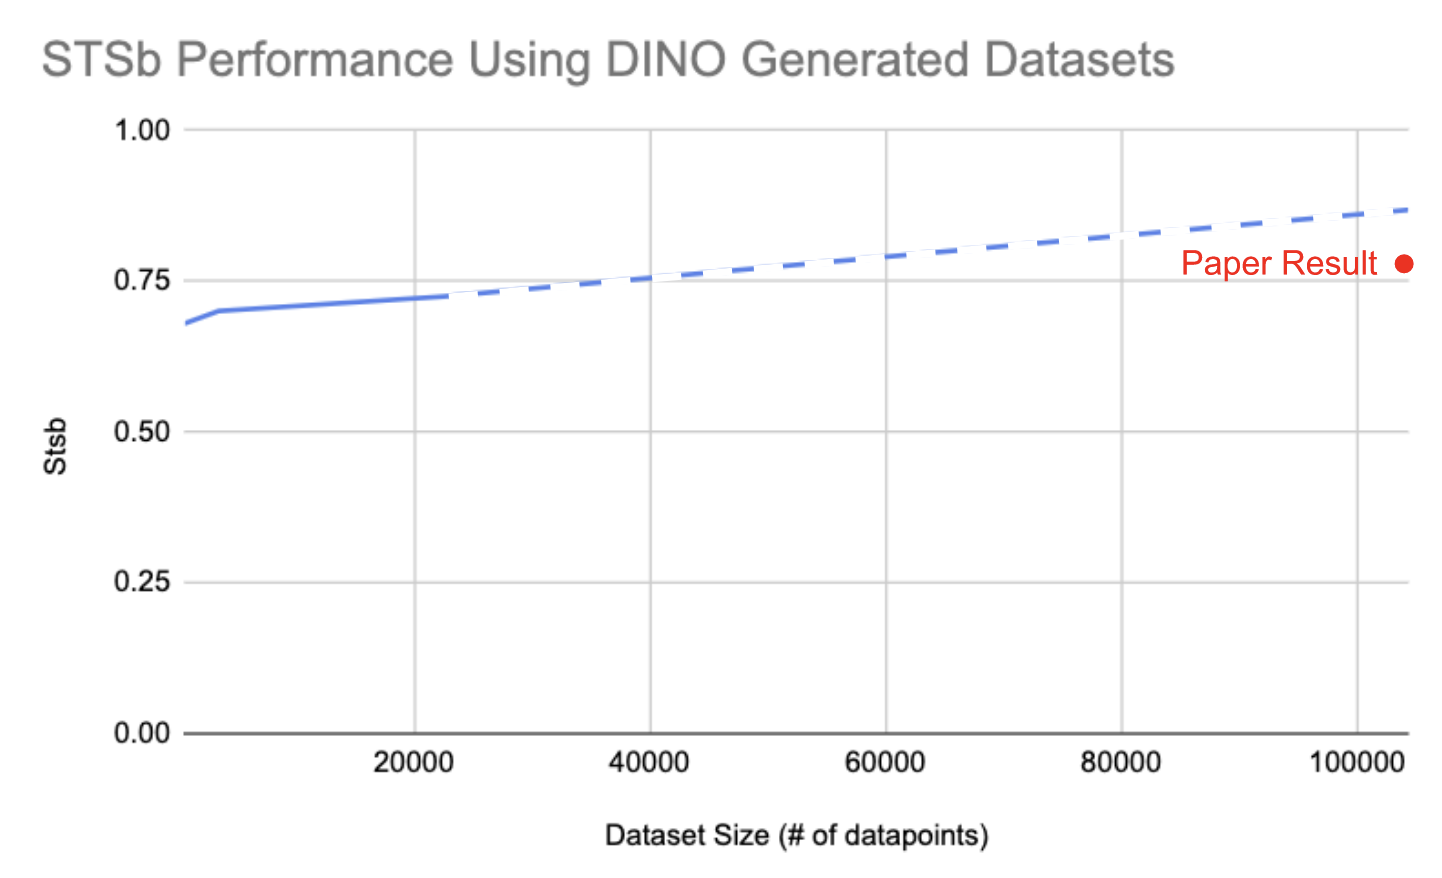
\includegraphics[width=0.99\linewidth]{DINO_STS_NEW.png}
    \caption{STSb Performance Using DINO-Generated Textual Similarity Datasets}
    \label{fig:repcurve}
\end{figure}


\subsection{News Headline Classification}

Next, we retool DINO to a new task: that of news headline classification. For this task, given a news headline, the model must classify it under the topic it discusses. We use the \textit{ag\_news} dataset from Hugging Face as the real dataset against which to benchmark. This dataset contains 120K headlines separated into four categories: world, sports, business, and science. We use the DINO approach with the instructions given in Table \ref{tab:instructions} to prompt GPT2-large to generate news headlines about the topics corresponding to the labels of the Hugging Face \textit{ag\_news} dataset. We generate two datasets in this manner using different sets of prompts, which we term "naive" and "human".  

Each of these instruction sets was used with GPT2-large to generate a headline dataset of size 6.2K. In addition to the two DINO-generated datasets, we uniformly sampled examples from each of the categories from the original \textit{ag\_news} dataset for the "real" benchmark dataset to obtain a total of 6.2k headlines to make the comparison fair. 

\begin{table*}[h]
    \centering
    \begin{tabular}{c|c}
        \textbf{\textit{DINO-naive} instructions} & \textbf{\textit{DINO-human} instructions} \\
        \hline
        Write a world news headline & Write a headline about international incidents \\
        & Write a headline about international politics \\
        Write a sports news headline & Write an Olympic sports news headline \\
        & Write a national sports news headline \\
        Write a business news headline & Write a news headline about financial institutions \\
        & Write a news headline about corporations \\
        Write a science news headline & Write a science news headline \\
        & Write a technology news headline \\
    \end{tabular}
    \caption{Instruction sets, or prompts to the PLM.}
    \label{tab:instructions}
\end{table*}

The two DINO-generated datasets were created using different sets of prompts, shown in Table \ref{tab:instructions}. For the first ("naive"), we modeled the prompts directly off those for the sentence similarity dataset. We observed that the sentences generated by these prompts lacked nuance, and were unrelated to the target category at times. For example, sentences generated for the business category prompt included "I'm going to start my own company!" and "I'm going to start my own business." As can be seen, these lack diversity and are quite generic. Therefore, we also developed a second set of prompts ("human") through empirically testing what wordings of prompts generated more realistic outputs. We noticed that the business news headlines generated by the naive prompts were particularly bad, whereas the other categories were more acceptable. Therefore, we changed the prompts for business news more drastically than for the others. To e nable more specificity, we split each category into two more specific sub-categories, and post-processed the data to combine the subcategories. 

After generating the three datasets (\textit{ag\_news}, \textit{DINO-naive}, \textit{DINO-human}), we fine-tune three DistilBERT models on the datasets and compare their performances on headline classification.



\section{Results}

\subsection{Performance Analysis}

After fine-tuning the DistilBERT model on the three separate datasets, we observe the accuracy of the models evaluated on a held out validation dataset from \textit{ag\_news} (see Figure \ref{fig:maxvalacc}). We find that the model fine-tuned on the \textit{ag\_news} dataset performs the best. The model fine-tuned on the \textit{DINO-human} dataset performs very close to the \textit{ag\_news} data, while the naive dataset performs significantly worse.

\begin{figure}[]
    \centering
    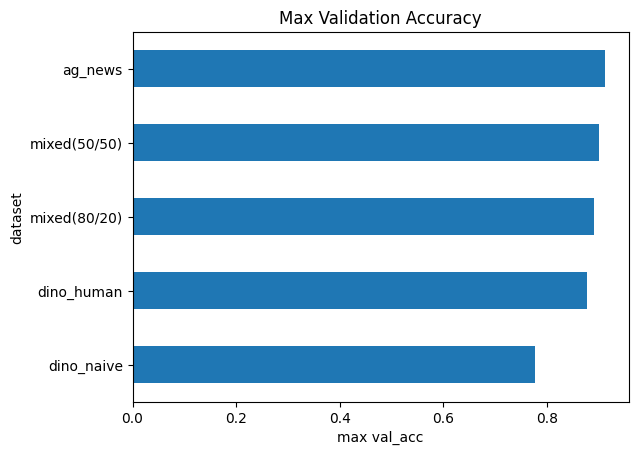
\includegraphics[width=0.99\linewidth]{Accuracy Bar Graph.png}
    \caption{Maximum validation accuracy of DistilBERT fine-tuned on each dataset}
    \label{fig:maxvalacc}
\end{figure}

To uncover why these differences exist, we plot the validation accuracy for all three models over the two epochs of training (Figure \ref{fig:Acccuracy Curves.png}). We observed that the model trained on \textit{ag\_news} continues to improve over training, with its test accuracy steadily increasing as the training epochs progress. However, the model trained on the \textit{DINO-human} dataset shows much slower improvement, such that the performance gap between the model trained on \textit{DINO-human} and the model trained on \textit{ag\_news} grows over training. And for the model trained on the \textit{DINO-naive} dataset, we find that its test accuracy increases for a while but then actually decreases as the training epochs grows.

\begin{figure}[]
    \centering
    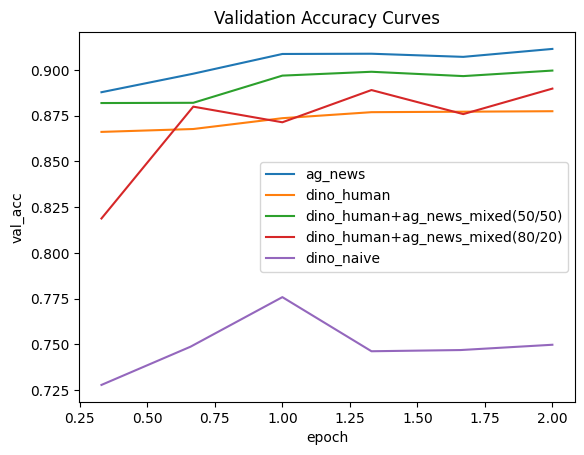
\includegraphics[width=0.99\linewidth]{Accuracy Curves.png}
    \caption{Validation Accuracy vs Epoch of DistilBERT fine-tuned on each dataset}
    \label{fig:Acccuracy Curves.png}
\end{figure}

Based on these results, we suspect that the models fine-tuned on the DINO-generated datasets are overfitting. We plot the training and validation loss curves of the model trained on each of the three different datasets. In the loss curves of the model fine-tuned on the \textit{ag\_news} dataset, we observe that both losses are monotonically decreasing. We also observe that the training loss does not immediately go to zero, but steadily decreases as the epochs grow (Figure \ref{fig:threelosscurves}). This suggests that the model fine-tuned on the \textit{ag\_news} dataset is not overfitting. When we look at the loss curves of the model trained on \textit{DINO-naive} and \textit{DINO-human}, we see that the validation loss does not monotonically decrease. In the case of the model trained on \textit{DINO-naive}, the test loss actually increases significantly during a period of training. We also observe that the models trained on both DINO datasets exhibit the same pattern in the training loss: it decreases extremely rapidly to near zero and stays there (Figure \ref{fig:threelosscurves}). This suggests that the models trained on the DINO generated datasets saturate extremely quickly, and thus are overfitting.

\begin{figure}[t]
    \centering
    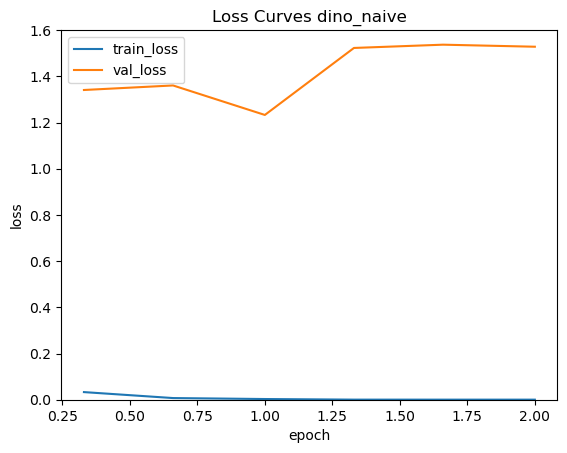
\includegraphics[width=0.85\linewidth]{naivecurve.png}
    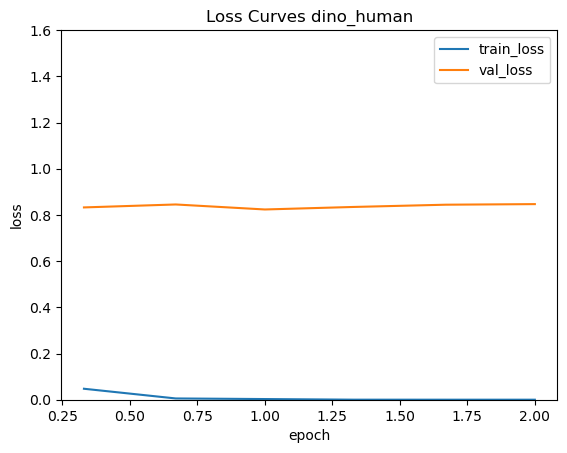
\includegraphics[width=0.85\linewidth]{humancurve.png}
    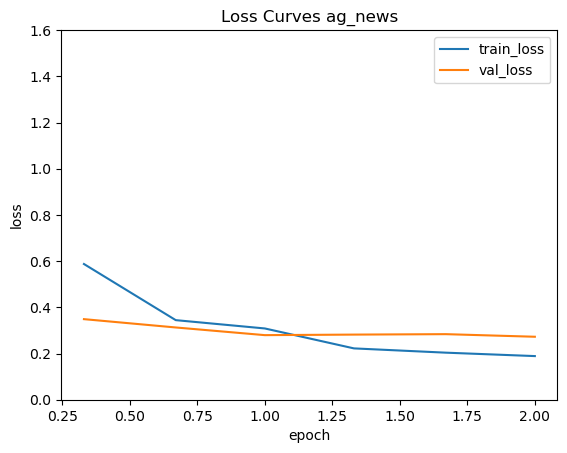
\includegraphics[width=0.85\linewidth]{agcurve.png}
    \caption{Loss curves for models fine-tuned on \textit{ag\_news}, \textit{DINO-naive}, and \textit{DINO-human}}
    \label{fig:threelosscurves}
\end{figure}

This seems to suggest fundamentally different data distributions between the real news headlines and the DINO generated ones: despite the fact that the \textit{DINO-human} dataset increases the test performance of the model significantly, it still exhibits the same overfitting behavior as the \textit{DINO-naive} dataset. The real data \textit{ag\_news} has the desirable property that better performance is gained by additional training epochs, that the DINO-generated datasets do not. 



\subsection{Dataset Analysis}

We are interested in understanding the differences between the datasets quantitatively and qualitatively.

We start by looking at the confusion matrices of the models trained on the \textit{DINO-naive} and \textit{ag\_news} datasets and evaluated on the validation set from \textit{ag\_news} (for the confusion matrices of the models trained on the other datasets, see the Appendix). Figures \ref{fig:confusion1} \& \ref{fig:confusion2} reveal that the model fine-tuned on the \textit{DINO-naive} datasets performs much worse on business news. This is supported when we inspect that \textit{DINO-naive} dataset. We find that many of the generated business headlines are poor in quality, as exhibited by the examples below:
\begin{itemize}
    \item "I have a business problem"
    \item "I'm going to start a company."
    \item "This company has a new product, so I'm going to tell my coworkers about it. I want them to be excited about what they see."
\end{itemize}

\begin{figure}[h]
    \centering
    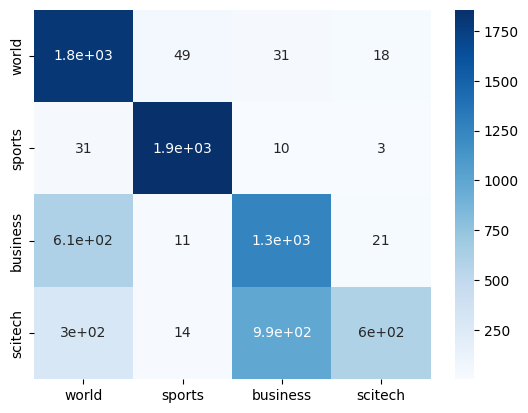
\includegraphics[width=0.8\linewidth]{cm_naive.png}
    \caption{\textit{DINO-naive} confusion matrix}
    \label{fig:confusion1}
    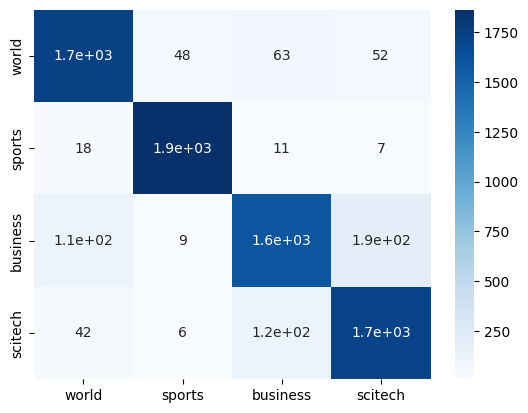
\includegraphics[width=0.8\linewidth]{cm_real.png}
    \caption{\textit{ag\_news} confusion matrix}
    \label{fig:confusion2}
\end{figure}

Inspecting the \textit{DINO-naive} dataset, we also notice a pattern in the generated data: many of the headlines share a prefix. For example, consider the following excerpt from the \textit{DINO-naive} dataset:
\begin{itemize}
    \item " \textbf{A new method for detecting cancer cells} from a single DNA sequence"
    \item "\textbf{A new method for detecting cancer cells} using a single drop of urine"
    \item "\textbf{A new method for detecting cancer cells} using an optical technique"
    \item "\textbf{A new method for detecting cancer} from DNA in a living organism"
\end{itemize}

We hypothesize that this is due to the autoregressive manner in which text is sampled from GPT: since tokens are generated one at a time, this naturally makes the generated text share prefixes. \footnote{We note that this may be resolved by increasing the temperature parameter when sampling tokens} Based on this observation, we suspect that the DINO-generated datasets may have less informational content than the \textit{ag\_news} dataset because the generated headlines share many redundancies. This could explain why the models fine-tuned on the generated data exhibit overfitting: despite all datasets having the same number of headlines, the DINO-generated datasets are functionally "smaller" in real information that the model can learn from.

We performed some quantitative analysis on the datasets. Looking at the distribution of headline length (Figure \ref{fig:violin}) we find that there is not much difference in headline length between the DINO-generated datasets (with the mean and overall histogram looking very similar). The \textit{ag\_news} dataset exhibits a significantly higher headline length than the DINO-generated datasets, with the mean being the same as the max length of the synthetic datasets. \footnote{We note that there is a parameter in DINO that controls the maximum length of generated texts that can be modified to produce longer headlines}

Looking at the number of unique tokens (tokens being words) in each dataset, we find that the \textit{ag\_news} dataset contains almost an order of magnitude more unique words than the generated datasets. We find that the \textit{DINO-human} dataset has more unique tokens than \textit{DINO-naive}, although not by much (Table \ref{tab:unique_tokens}).

\begin{figure}[t]
    \centering
    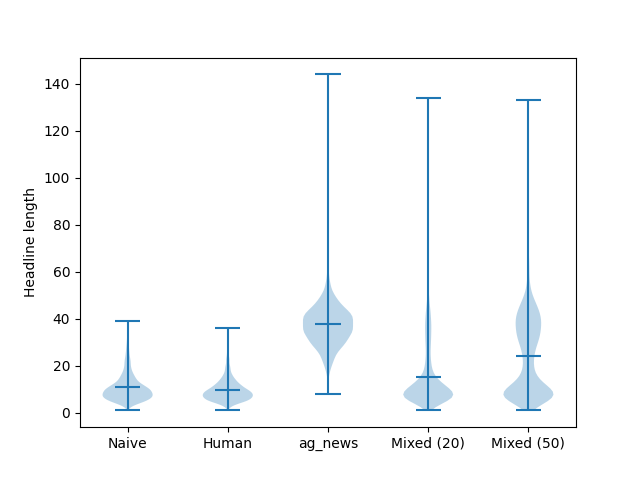
\includegraphics[scale=0.5]{figures/violin_plots.png}
    \caption{The length of headlines in words. The width represents the density (i.e., how many headlines in that dataset were of the given length). The three horizontal markers represent the min, max and mean length of headlines.}
    \label{fig:violin}
\end{figure}

\begin{table}[h]
    \centering
    \begin{tabular}{c|c}
        Dataset & Num Unique Tokens \\ \hline
        Naive & 5964 \\ 
        Human & 6388 \\
        Mixed (20) & 13826 \\
        Mixed (50) & 19874 \\
        \textit{ag\_news} & 27911
    \end{tabular}
    \caption{Number of Unique Tokens (words)}
    \label{tab:unique_tokens}
\end{table}

Interestingly, we note that the quantitative differences between the \textit{DINO-naive} and \textit{DINO-human} datasets are minimal, but the performance of the model trained on \textit{DINO-human} is significantly better. This suggests that the improve in dataset quality of \textit{DINO-human} is in some aspect unrelated to the length or diversity in tokens. This supports our original intuition in creating the \textit{DINO-human} dataset: the prompts matter a lot in improving the quality of the dataset, beyond just increasing the size or diversity (in tokens). This is easily demonstrated by inspecting the datasets qualitatively. We pull a headline about the financial market from all three datasets to compare:

\begin{itemize}
    \item \textit{DINO-naive}: "I just bought some stock."
    \item \textit{DINO-human}: "FED-Backed Bank Feds Shut Down \$2B of Assets"
    \item \textit{ag\_news}: "Fed President Calls Oil Troublesome Record oil prices" are creating headwinds for the U.S. economy but do not place its recovery at risk, Dallas Federal Reserve Bank President Robert McTeer said on Monday."
\end{itemize}

We see that our small change in prompts greatly improves the quality of the generated dataset, though it is still far from the real headline in complexity or detail.


\subsection{Mixed datasets analysis}

Given the fundamental difference in loss curve shapes that were observed between the model trained on the \textit{ag\_news} dataset and the ones trained on the DINO-generated datasets, we created a new dataset which combined some of the headlines from the real dataset with those from \textit{DINO-human}, and trained a model on this mixed dataset. To keep the size of the dataset and the number of headlines per label consistent, for every DINO-generated headline sampled at random, we substitute it for an \textit{ag\_news} headline from the same topic.

When we switch out only 20\% of the DINO-generated data with the original data, the shape of the loss curves changes dramatically. Not only does the gap between the train loss and validation loss decrease on average, but the train loss also decreases over the epochs and the validation loss starts to decrease before stabilizing around 0.39 (Figure \ref{fig:mixedloss}). 

\begin{figure}
    \centering
    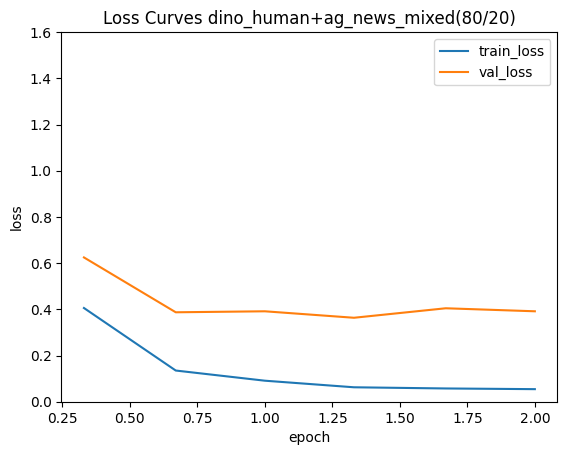
\includegraphics[width=0.9\linewidth]{figures/mixed_dataset_80:20.png}
    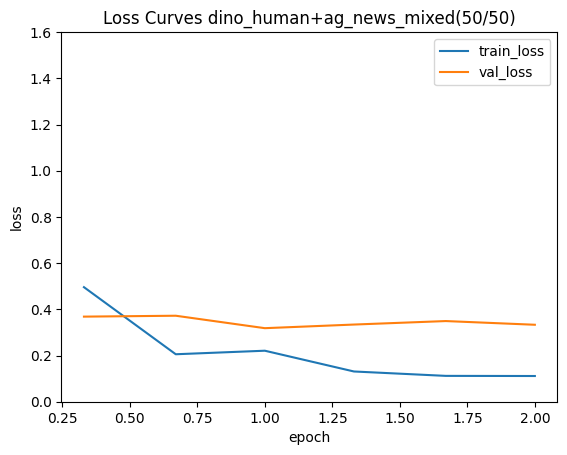
\includegraphics[width=0.9\linewidth]{figures/mixed_dataset_50 50.png}
    \caption{Loss Curves for Mixed Datasets}
    \label{fig:mixedloss}
\end{figure}

When we substitute 50\% of the DINO-generated headlines with real headlines, we find that both the train and the validation loss curves for the new dataset looks very similar to the \textit{ag\_news} dataset (Figure \ref{fig:threelosscurves} \& \ref{fig:mixedloss}).

From this experiment, we demonstrate that datasets composed of a mix of DINO-generated data and real data can also perform quite well. This could prove very helpful for settings where there is data available but not in sufficient quantity, or for data augmentation, provided that prompts of strong enough quality can be written.


\section{Conclusion}

Datasets generated with PLMs using the DINO approach exhibit reasonable promise -- we have shown that models trained on them are able to achieve performance close to that of models trained on real datasets. We note that the wording of the prompting given to the PLM is of great importance, and demonstrate that through comparing datasets generated with two different sets of prompts. A weakness of the generated datasets is their tendency towards redundancy, which is problematic because diversity in data reduces overfitting. This can be mitigated by improving the prompts and tuning the generation model's hyperparameters.




\section*{Limitations}

The experiments conducted were on a smaller scale (e.g. 6K headlines in the generated datasets). \footnote{We were limited by computational resources, in particular GPUs} Reproducing these results on a much larger scale would be valuable.

Also, after observing the statistics of the data, particularly the average length of the generated headlines and noticing that the DINO-generated headlines were on average shorter than the ones from \textit{ag\_news}, we discovered that the script created by \citet{schick2021generating} to generate data using the DINO approach had a default maximum output length value of 40. Given more time, we would explore whether a higher upper bound on the length of generation would improve the generations and thereby improve the performance of the trained model, or whether longer sequences would be more likely to generate nonsensical content.

Additionally, since the validation data we used to evaluate the three datasets was the \textit{ag\_news} validation dataset, the results could be biased towards the model trained on the \textit{ag\_news} train data. Although the \textit{ag\_news} validation dataset contains different headlines than its training dataset, the data is still sampled from the same distribution. This could have contributed towards the model trained on the \textit{ag\_news} data outperforming the models trained on the DINO-generated data. Future work could examine the performance of the models on an existing news dataset other than \textit{ag\_news} to see if the difference in accuracy percentage of the different models would remain consistent.

It would also be interesting to see the value of our methods for dataset augmentation. This could be done by training a model on a small real dataset, and then augmenting the dataset using our method DINO and training a model on that mixed dataset, and comparing the performances. (Our analyses were all performed on datasets of equal size.)

Finally, further experimentation with the prompts given to the PLM as well as tweaking the parameters of the model, for example the temparature, could also yield interesting results.


\bibliographystyle{acl_natbib}
\bibliography{ref}


\appendix

\section{Appendix}
\label{sec:appendix}

Our code and datasets are available at: \url{https://github.com/jasony123123/dino.git}. \\

This represents our own work in accordance with University regulations.
\\
$\backslash$s$\backslash$ Nada Elfazary\\
$\backslash$s$\backslash$ Katie Baldwin\\
$\backslash$s$\backslash$ Jason Yuan\\

\clearpage

\textbf{Confusion matrices of remaining datasets}

\begin{figure}[h]
    \centering
    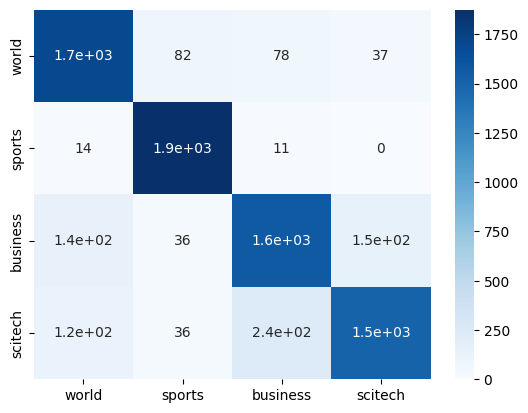
\includegraphics[width=0.8\linewidth]{figures/cm_human.png}
    \caption{DINO-Human dataset confusion matrix}
\end{figure}
\begin{figure}[h]
    \centering
    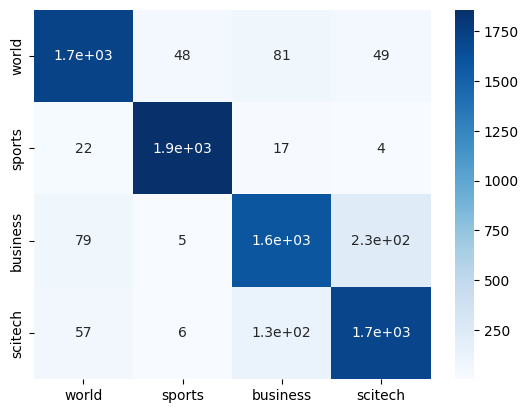
\includegraphics[width=0.8\linewidth]{figures/cm_mixed_data20.png}
    \caption{Mixed 20/80 dataset confusion matrix}
\end{figure}
\begin{figure}[h]
    \centering
    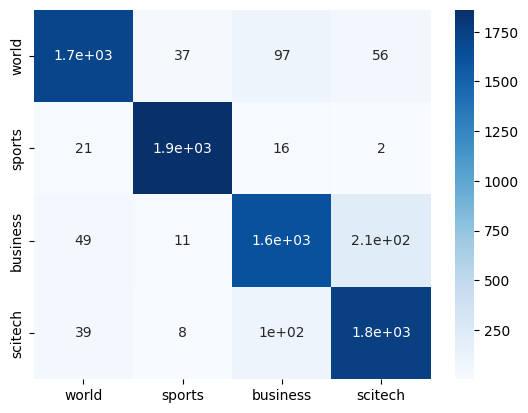
\includegraphics[width=0.8\linewidth]{figures/cm_mixed_dataset_50.png}
    \caption{Mixed 50/50 dataset confusion matrix}
\end{figure}


\end{document}

